
\chapter[Lý thuyết và bài tập: Dao động tắt dần, dao động duy trì, dao động cưỡng bức;\\Lý thuyết và bài tập: Hiện tượng cộng hưởng]{Lý thuyết và bài tập: Dao động tắt dần, dao động duy trì, dao động cưỡng bức;\\Lý thuyết và bài tập: Hiện tượng cộng hưởng}
\section{Lý thuyết}
\subsection{Dao động tắt dần}
\subsubsection{Thế nào là dao động tắt dần?}
Dao động tắt dần là dao động có biên độ giảm dần theo thời gian.
\subsubsection{Nguyên nhân gây ra dao động tắt dần}
Khi con lắc dao động, nó chịu lực cản (lực ma sát) làm tiêu hao cơ năng của con lắc. Vì thế, biên độ dao động của con lắc giảm dần và cuối cùng con lắc dừng lại.
\subsubsection{Ứng dụng}
Các thiết bị đóng cửa tự động hay bộ phận giảm xóc của ô tô, xe máy, ... là những ứng dụng của dao động tắt dần.

Chú ý rằng dao động tắt dần càng nhanh nếu lực cản của môi trường càng lớn.
\begin{center}
	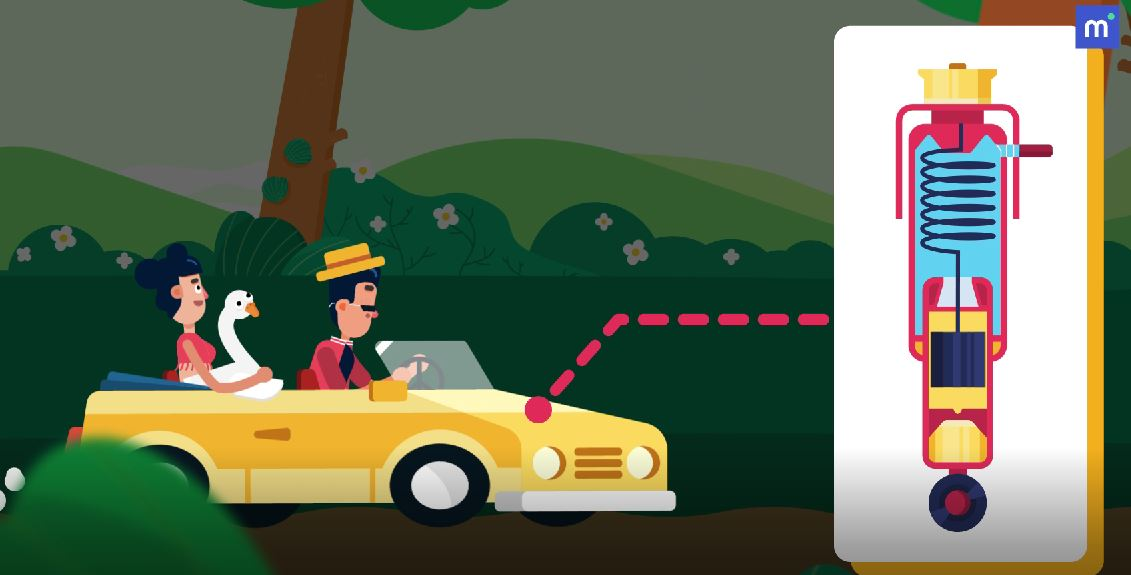
\includegraphics[scale=0.5]{../figs/VN12-PH-05-L-004-1-V2-03}
\end{center}
\subsection{Dao động duy trì}
\subsubsection{Thế nào là dao động duy trì?}
Nếu ta cung cấp thêm năng lượng cho vật dao động tắt dần (do ma sát) để bù lại sự tiêu hao vì ma sát mà không làm thay đổi chu kì riêng của nó thì dao động kéo dài mãi mãi và được gọi là dao động duy trì.
\subsubsection{Ví dụ về dao động duy trì}
Dao động của con lắc đồng hồ là dao động duy trì.
\begin{center}
	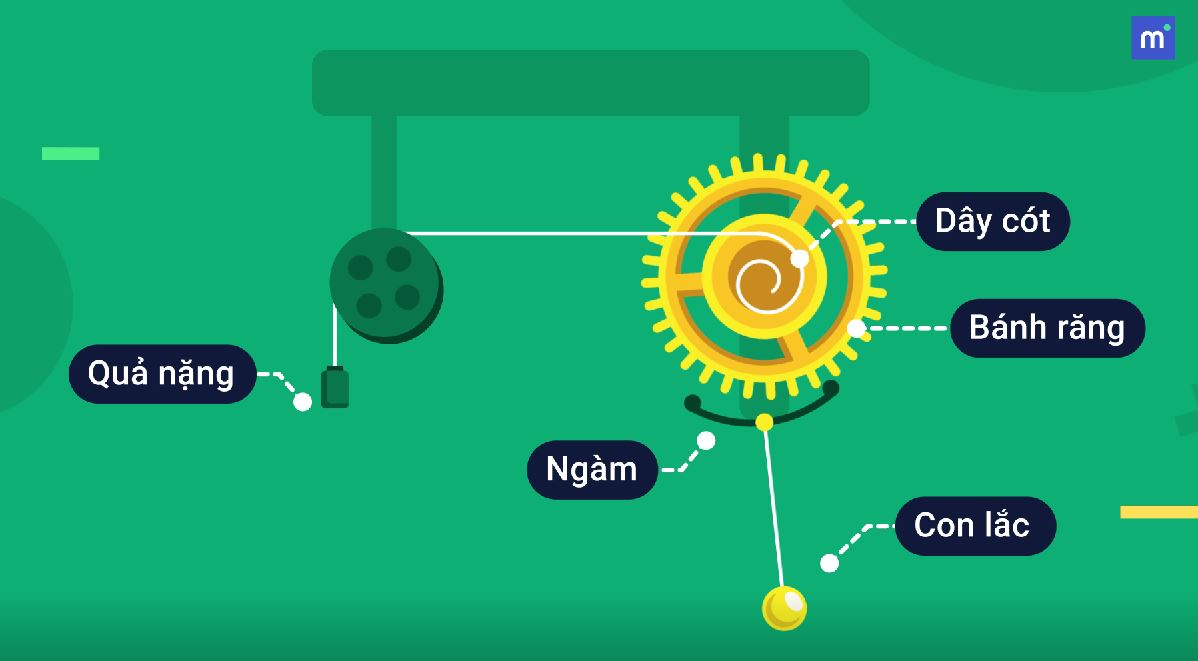
\includegraphics[scale=0.3]{../figs/VN12-PH-05-L-004-1-V2-01}
\end{center}
\subsection{Dao động cưỡng bức}
\subsubsection{Thế nào là dao động cưỡng bức?}
Dao động cưỡng bức là dao động chịu tác dụng của một ngoại lực cưỡng bức tuần hoàn với tần số $f$ để bù lại phần năng lượng mà hệ tiêu hao do ma sát.
\subsubsection{Ví dụ về dao động cưỡng bức}
Dao động cưỡng bức gây ra bởi xylanh trong động cơ xe lên thân xe, làm cho thân xe dao động.
\subsubsection{Đặc điểm}
\begin{enumerate}[label=\alph*)]
	\item Dao động cưỡng bức có biên độ $A$ không đổi và có tần số bằng tần số của lực cưỡng bức ($f_{\text {cb}}=f$);
	\item Biên độ của dao động cưỡng bức tỉ lệ thuận với biên độ của lực cưỡng bức và phụ thuộc vào độ chênh lệch giữa tần số của lực cưỡng bức và tần số riêng của hệ dao động. Khi tần số của lực cưỡng bức càng gần tần số riêng thì biên độ dao động cưỡng bức càng lớn.
\end{enumerate}
\begin{center}
	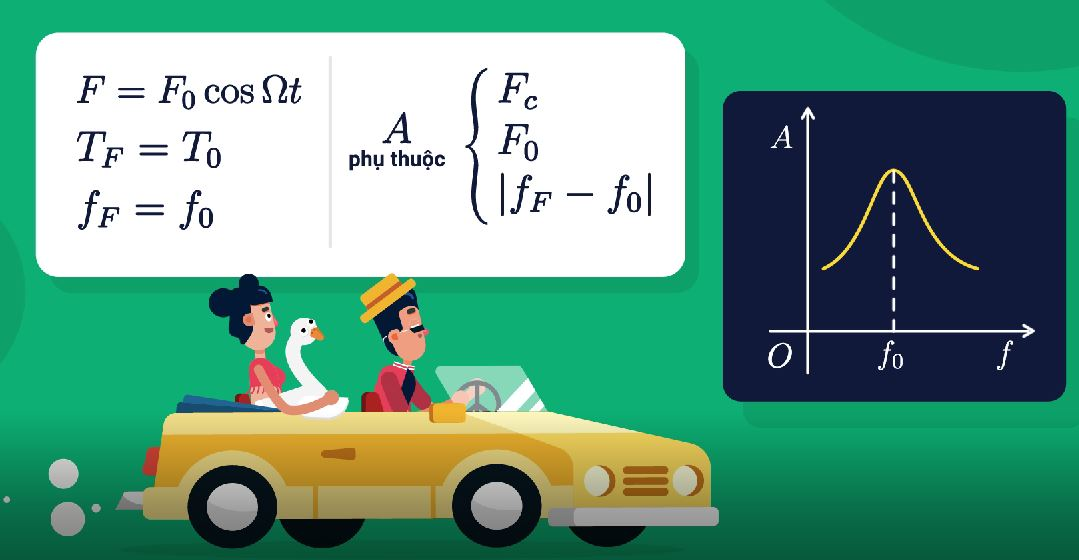
\includegraphics[scale=0.5]{../figs/VN12-PH-05-L-004-1-V2-02}
\end{center}
\subsection{Phân biệt dao động cưỡng bức với dao động duy trì}
\subsubsection{Giống nhau} 
\begin{itemize}
	\item Đều tác dụng \bltext{ngoại lực} vào hệ.
	\item Đều cung cấp \bltext{năng lượng} làm cho dao động của hệ không bị \bltext{tắt dần}.
\end{itemize}
\subsubsection{Khác nhau}
Dao động cưỡng bức buộc hệ phải dao động theo \bltext{tần số của ngoại lực cưỡng bức}. Dao động duy trì chỉ cung cấp năng lượng, không làm thay đổi \bltext{tần số dao động của hệ}. 
\subsubsection{Thế nào là hiện tượng cộng hưởng?}
Hiện tượng biên độ dao động cưỡng bức tăng đến giá trị cực đại khi tần số $f$ của lực cưỡng bức tiến đến bằng tần số riêng $f_0$ của hệ dao động gọi là hiện tượng cộng hưởng.
\begin{center}
	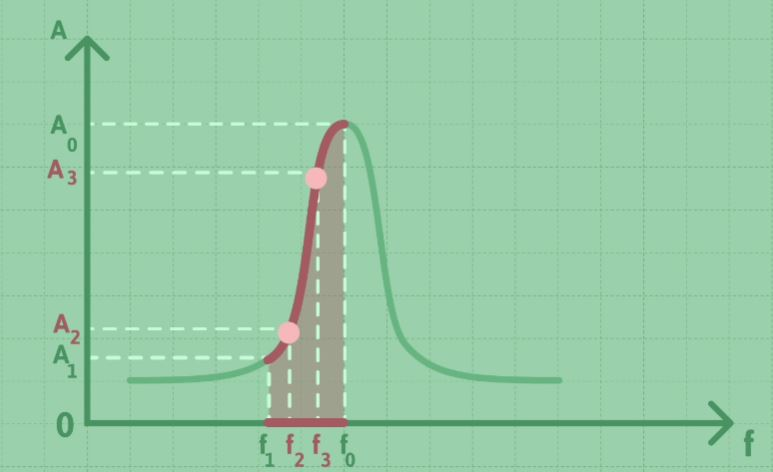
\includegraphics[scale=0.5]{../figs/VN12-PH-05-L-004-2-V2-01.jpg}
\end{center}
\subsubsection{Điều kiện cộng hưởng}
\begin{itemize}
	\item Hệ có dao động cưỡng bức;
	\item Tần số của lực cưỡng bức \bltext{bằng} tần số riêng của hệ ($f=f_0$).
\end{itemize}
\subsubsection{Đặc điểm}
Khi lực cản của môi trường nhỏ thì hiện tượng cộng hưởng rõ nét (đồ thị cộng hưởng nhọn), khi lực cản của môi trường lớn thì hiện tượng cộng hưởng không rõ nét (đồ thị cộng hưởng tù).
\subsubsection{Ứng dụng}
Hộp cộng hưởng của đàn guitar, violon,...
\begin{center}
	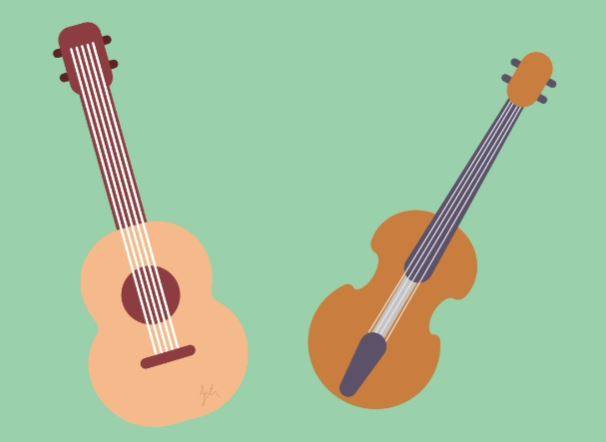
\includegraphics[scale=0.5]{../figs/VN12-PH-05-L-004-2-V2-02.jpg}
\end{center}
\section{Mục tiêu bài học - Ví dụ minh họa}
\begin{dang}{Nhận biết được dao động tắt dần,\\ dao động cưỡng bức, dao động duy trì}
	\viduii{1}{Dao động duy trì dao động xảy ra dưới tác dụng của ngoại lực tuần hoàn có tần số
		\begin{mcq}
			\item bằng tần số của dao động tự do.
			\item bất kỳ.
			\item bằng nửa tần số của dao động tự do.
			\item bằng 2 lần tần số của dao động tự do.
		\end{mcq}
	}
	{\begin{center}
			\textbf{Hướng dẫn giải}
		\end{center}
		
		Dao động duy trì là dao động xảy  ra dưới tác dụng của ngoại lực tuần hoàn có tần số bằng tần số của dao động tự do.
		
		\textbf{Đáp án: A.}
	}
	\viduii{1}{Khi nói về dao động cưỡng bức, phát biểu nào sau đây là đúng?
		\begin{mcq}
			\item Dao động của con lắc đồng hồ là dao động cưỡng bức.
			\item Biên độ của dao động cưỡng bức là biên độ của lực cưỡng bức.
			\item Dao động cưỡng bức có biên độ không đổi và có tần số bằng tần số của lực cưỡng bức.
			\item Dao động cưỡng bức có tần số nhỏ hơn tần số của lực cưỡng bức.
		\end{mcq}
	}
	{\begin{center}
			\textbf{Hướng dẫn giải}
		\end{center}
		
		A. đúng vì dao động của con lắc đồng hồ là dao động cưỡng bức.
		
		B. sai vì biên độ của dao động cưỡng bức phụ thuộc vào tần số ngoại lực tỉ lệ với biên độ của ngoại lực.
		
		C. sai vì dao động cưỡng bức có biên độ thay đổi và đạt cực đại khi tần số lực cưỡng bức bằng tần số riêng
		
		D. sai vì dao động cưỡng bức có tần số chính là tần số của lực cưỡng bức.
		
		\textbf{Đáp án: A.}
	}
	\viduii{1}{Một vật dao động tắt dần có các đại lượng giảm liên tục theo thời gian là
		\begin{mcq}(2)
			\item biên độ và gia tốc.
			\item li độ và tốc độ.
			\item biên độ và năng lượng.
			\item biên độ và tốc độ.
		\end{mcq}
	}
	{\begin{center}
			\textbf{Hướng dẫn giải}
		\end{center}
		
		Theo định nghĩa về dao động tắt dần thì biên độ và năng lượng giảm liên tục theo thời gian.	
		
		\textbf{Đáp án: C.}
	}
\end{dang}
\begin{dang}{Phân biệt được dao động tắt dần,\\ dao động duy trì, dao động cưỡng bức}
	\ppgiai{
		\textbf{Bài toán về năng lượng trong dao động tắt dần}
		
		Cơ năng 
		\begin{equation*}
			W=\dfrac{1}{2}kA^2.
		\end{equation*}
		Mối quan hệ giữa độ giảm năng lượng và độ giảm biên độ sau 1 chu kì:
		
		Ta có: 
		\begin{equation*}
			\dfrac{W'}{W}=\left( \dfrac{A'}{A}\right) ^2\Rightarrow \dfrac{\Delta W}{W}=1-\left( \dfrac{A'}{A}\right) ^2=\dfrac{\left( A+A'\right)\left( A-A'\right)  }{A^2}.
		\end{equation*}
		Làm gần đúng:
		\begin{equation*}
			A+A'=2A\Rightarrow \dfrac{\Delta W}{W}=\dfrac{2\Delta A}{A}.
		\end{equation*}
		Phần trăm biên độ bị giảm sau n chu kì:
		\begin{equation*}
			\dfrac{A-A_\text{n}}{A}.
		\end{equation*}
		Phần trăm cơ năng còn lại sau n chu kì:
		\begin{equation*}
			\dfrac{W_\text{n}}{W}=\left( \dfrac{A_\text{n}}{A}\right) ^2. 
		\end{equation*}
		Sau 1 chu kì biên độ giảm a\% thì sau n chu kì biên độ của vật là: 
		\begin{equation*}
			A_\text{n}=\left( 1-a\%\right)^\text{n}A.
		\end{equation*}
	}
	\viduii{3}{Một con lắc dao động tắt dần. Cứ sau mỗi chu kì, biên độ giảm $\SI{3}{\percent}$. Phần năng lượng của con lắc bị mất đi trong một dao động toàn phần là bao nhiêu?
		\begin{mcq}(4)
			\item $\SI{3}{\percent}$.
			\item $\SI{6}{\percent}$.
			\item $\SI{4.5}{\percent}$.
			\item $\SI{9}{\percent}$.
		\end{mcq}
	}
	{\begin{center}
			\textbf{Hướng dẫn giải}
		\end{center}
		
		Giả sử biên độ ban đầu là $A$.
		
		Sau một chu kỳ biên độ con lắc còn $A_1=\text{0,97}A$.
		\begin{equation*}
			\Rightarrow \dfrac{W_\text{1}}{W}=\left( \dfrac{A_\text{1}}{A}\right) ^2=\text{0,97}^2.
		\end{equation*}
		Phần trăm cơ năng con lắc bị mất đi trong hai dao động toàn phần liên tiếp là:
		\begin{equation*}
			\dfrac{\Delta W_\text{1}}{W}=1-\text{0,97}^2\approx 6\%.
		\end{equation*}
		
		\textbf{Đáp án: B.}
		
	}
	\viduii{3}{Một con lắc lò xo dao động tắt dần trên mặt phẳng nằm ngang. Cứ sau mỗi chu kì biên độ giảm 2\%. Gốc thế năng tại vị trí mà lò xo không bị biến dạng. Phần trăm cơ năng con lắc bị mất đi trong hai dao động toàn phần liên tiếp có giá trị gần nhất với giá trị nào sau đây?
		\begin{mcq}(4)
			\item  7\%.
			\item  4\%.
			\item 10\%.
			\item 8\%.
		\end{mcq}
	}
	{\begin{center}
			\textbf{Hướng dẫn giải}
		\end{center}
		Giả sử biên độ ban đầu là $A$.
		
		Sau một chu kỳ biên độ con lắc còn
		\begin{equation*}
			A_1=\text{0,98}A.
		\end{equation*}
		Sau hai chu kỳ biên độ con lắc còn 
		\begin{equation*}
			A_2=\text{0,98}A_1=\text{0,98}^2A.
		\end{equation*}
		\begin{equation*}
			\Rightarrow \dfrac{W_\text{2}}{W}=\left( \dfrac{A_\text{n}}{A}\right) ^2=\text{0,98}^4.
		\end{equation*}
		Phần trăm cơ năng con lắc bị mất đi trong hai dao động toàn phần liên tiếp là:
		\begin{equation*}
			\dfrac{\Delta W_\text{2}}{W}=1-\text{0,98}^4\approx 8\%.
		\end{equation*}
		
		\textbf{Đáp án: D.}
	}
	\viduii{3}{
		Hai con lắc làm bằng hai hòn bi có bán kính bằng nhau, treo trên hai sợi dây có cùng độ dài. Khối lượng của hai hòn bi khác nhau. Hai con lắc cùng dao động trong một môi trường với li độ ban đầu như nhau và vận tốc ban đầu đều bằng 0. Dao động của con lắc nào tắt nhanh hơn: con lắc nặng hay con lắc nhẹ?
		\begin{mcq}
			\item con lắc nặng tắt nhanh hơn con lắc nhẹ tắt nhanh hơn còn tùy thuộc vào gia tốc trọng trường,
			\item hai con lắc tắt cùng một lúc.
			\item con lắc nhẹ tắt nhanh hơn.
			\item con lắc nặng tắt nhanh hơn.
		\end{mcq}
	}
	{\begin{center}
			\textbf{Hướng dẫn giải}
		\end{center}
		
		Cơ năng của con lắc tỉ lệ với khối lượng theo công thức: 
		\begin{equation*}
			W=\dfrac{1}{2}m \omega ^2 A^2.
		\end{equation*}
		Do cùng trong một môi trường nên lực ma sát tác dụng lên chúng trong mỗi chu kì như nhau. Con lắc nhẹ hơn có năng lượng ban đầu nhỏ hơn nên sẽ tắt nhanh hơn so với con lắc nặng.
		
		\textbf{Đáp án: C}.
	}
\end{dang}
\begin{dang}{Phát hiện được hiện tượng cộng hưởng.}
	\viduii{1}{Hiện tượng cộng hưởng cơ học xảy ra khi nào?
		\begin{mcq}
			\item Tần số của lực cưỡng bức bằng tần số của dao động cưỡng bức.
			\item Tần số dao động cưỡng bức bằng tần số dao động riêng của hệ.
			\item Tần số dao động cưỡng bức bằng tần số dao động riêng của hệ.
			\item Tần số của lực cưỡng bức bé hơn tần số riêng của hệ.
		\end{mcq}
	}
	{\begin{center}
			\textbf{Hướng dẫn giải}
		\end{center}
		Hiện tượng cộng hưởng xảy ra khi tần số của dao động cưỡng bức bằng với tần số dao động riêng của hệ.
		
		\textbf{Đáp án: B.}
	}
	\viduii{1}{Khi xảy ra hiện tượng cộng hưởng cơ thì vật tiếp tục dao động
		\begin{mcq}
			\item với tần số bằng tần số dao động riêng.
			\item với tần số nhỏ hơn tần số dao động riêng.
			\item với tần số lớn hơn tần số dao động riêng.
			\item mà không chịu ngoại lực tác dụng
		\end{mcq}
	}
	{\begin{center}
			\textbf{Hướng dẫn giải}
		\end{center}
		Khi xảy ra hiện tượng cộng hưởng cơ thì vật tiếp tục dao động với tần số bằng tần số dao động riêng.
		
		\textbf{Đáp án: A.}
	}
	
\end{dang}
\begin{dang}{Liên hệ các đặc điểm của hiện tượng\\ cộng hưởng để xác định điều kiện, biên độ, tần số khi xảy ra hiện tượng cộng hưởng.}
	\ppgiai{\begin{itemize}
			\item Hệ có dao động cưỡng bức;
			\item Tần số của lực cưỡng bức \bltext{bằng} tần số riêng của hệ (\bltext{$f=f_0$}).
		\end{itemize}
		
		Công thức tính chu kỳ con lắc lò xo $T=2\pi\sqrt{\dfrac{m}{k}}$, công thức tính chu kỳ con lắc đơn $T=2\pi\sqrt{\dfrac{l}{g}}$, công thức tính vận tốc $v=\dfrac{s}{t}$.}
	\viduii{2}{Một xe ô tô chạy trên đường, cứ cách $\SI{8}{\meter}$ lại có một cái mô nhỏ. Chu kì dao động tự do của khung xe trên các lò xo là $\SI{1.5}{\second}$. Xe chạy với vận tốc nào thì bị rung mạnh nhất?
		
		\begin{mcq}(2)
			\item $\SI{19.1}{\kilo \meter / \hour}.$
			\item $\SI{20.1}{\kilo \meter / \hour}.$
			\item $\SI{21.1}{\kilo \meter / \hour}.$
			\item $\SI{22.1}{\kilo \meter / \hour}.$
	\end{mcq}}
	{\begin{center}
			\textbf{Hướng dẫn giải}
		\end{center}
		
		Dao động của khung xe là dao động cưỡng bức, biên độ của dao động cưỡng bức sẽ lớn nhất khi xảy ra hiện tượng cộng hưởng. Tốc độ của xe để xảy ra hiện tượng cộng hưởng là
		\begin{equation*}
			T=\dfrac{l}{v} = T_0 \Leftrightarrow v= \dfrac{l}{T_0}=\dfrac {\SI{8}{\meter}}{\SI{1.5}{\second}} = \SI{5.3}{\meter / \second} = \SI{19.1}{\kilo \meter / \hour}.
		\end{equation*}
		Vậy khi ô tô chạy thẳng đều với tốc độ $v=\SI{19.1}{\kilo \meter / \hour}$ thì bị rung mạnh nhất.
		
		\textbf{Đáp án: A.}
	}
	\viduii{2}{	Một người đèo hai thùng nước ở phía sau xe đạp và đạp xe trên con đường lát bê tông. Cứ cách 
		3m, trên đường lại có một rãnh nhỏ. Đối với người đó tốc độ nào là không có lợi? Cho biết chu kì dao động riêng của nước trong thùng là $\text{0,6}\ \text{s}$.
		
		\begin{mcq}(4)
			\item $\SI{13}{\meter / \second}$.
			\item $\SI{14}{\meter / \second}$.
			\item $\SI{5}{\meter / \second}$.
			\item $\SI{6}{\meter / \second}$.
		\end{mcq}
	}
	{\begin{center}
			\textbf{Hướng dẫn giải}
		\end{center}
		Khi chu kì dao động riêng $T_0$ của nước bằng chu kì dao động cưỡng bức $T$ thì nước trong thùng dao động mạnh nhất, dễ đổ ra ngoài nhất nên không có lợi.
		\begin{equation*}
			T_0=T=\dfrac{s}{v}\Rightarrow v=\dfrac{s}{T_0}=\SI{5}{\meter / \second}.
		\end{equation*}
		
		\textbf{Đáp án: C.}
	}
	
\end{dang}